\documentclass[draft]{styles/agujournal2019}
\usepackage{url} 
\usepackage{lineno}

\usepackage{xr}
% Possible supplemental figures
\begin{figure}[]
    \setfigurenum{S1}
    \centering
    \begin{minipage}{0.5\textwidth}
        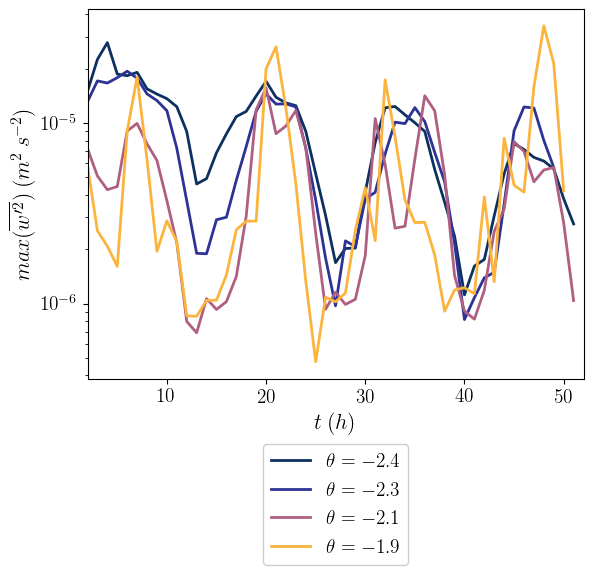
\includegraphics[width=\textwidth]{Figures/w2_max_cmp_dT_t.png}
    \end{minipage}%
    \begin{minipage}{0.5\textwidth}
        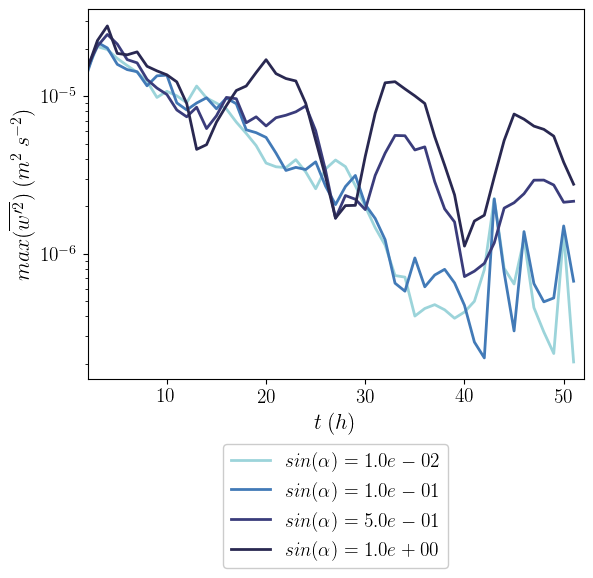
\includegraphics[width=\textwidth]{Figures/w2_max_cmp_dalpha_t.png}
    \end{minipage}
    \caption{Timeseries of maximum vertical velocity fluctuation per hour for (a) thermal driving cases and (b) slope cases.}
    \label{fig:max_w2_timeseries}
\end{figure}

\begin{figure}
    \centering
    \begin{minipage}{0.5\textwidth}
        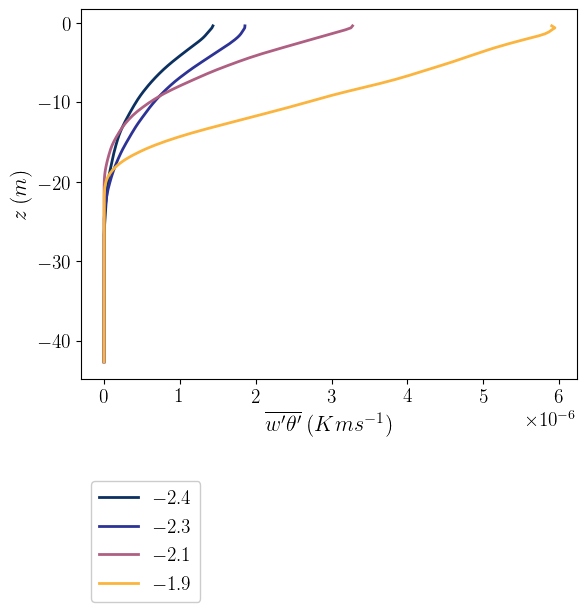
\includegraphics[trim={0 4cm 0 0},clip,width=\textwidth]{Figures/heatflux_cmp_dT_44h_tav12_z_profile.png}
    \end{minipage}%
    \begin{minipage}{0.5\textwidth}
        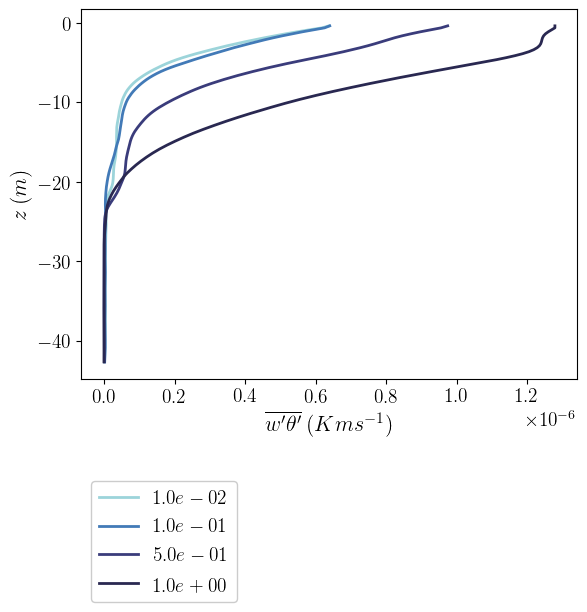
\includegraphics[trim={0 4cm 0 0},clip,width=\textwidth]{Figures/heatflux_cmp_slope_46h_tav12_z_profile.png}
    \end{minipage}
    \begin{minipage}{0.5\textwidth}
        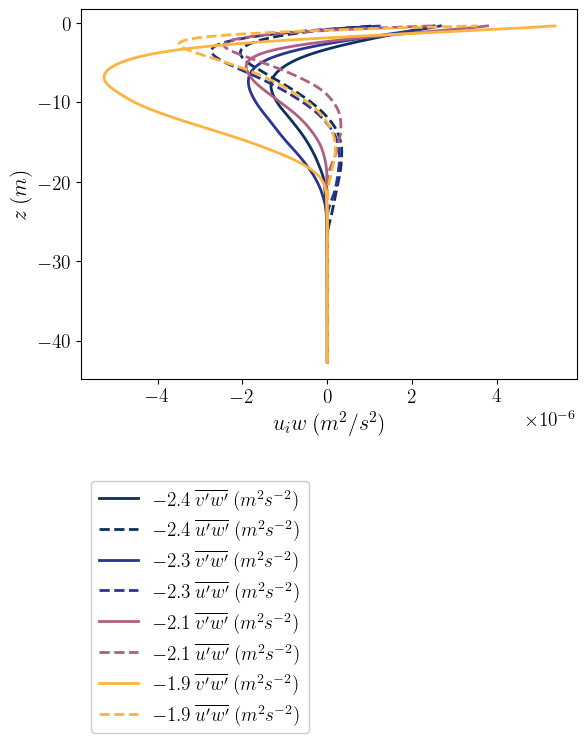
\includegraphics[trim={0 7.5cm 0 0},clip,width=\textwidth]{Figures/momflux_cmp_dT_44h_tav12_z_profile.png}
        \centering 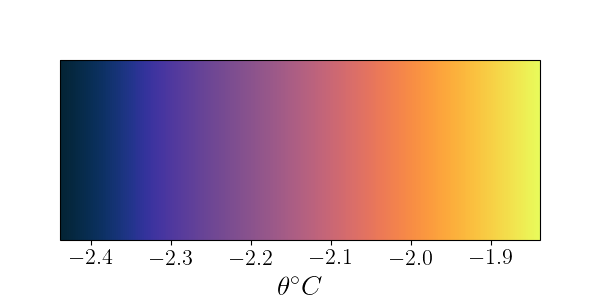
\includegraphics[width=0.7\textwidth,trim={1cm 0cm 1cm 5cm}, clip]{Figures/colorbar_thermal_driving.png}
    \end{minipage}%
    \begin{minipage}{0.5\textwidth}
        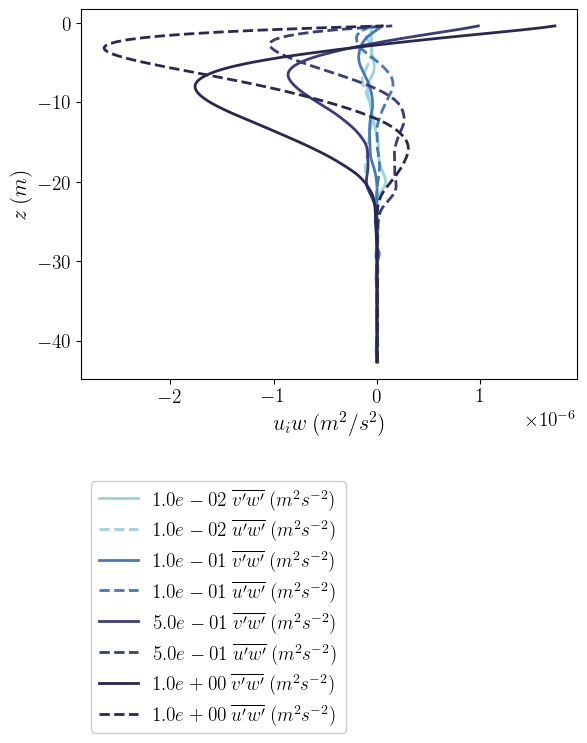
\includegraphics[trim={0 7.5cm 0 0},clip,width=\textwidth]{Figures/momflux_cmp_dslope_46h_tav12_z_profile.png}
        \centering 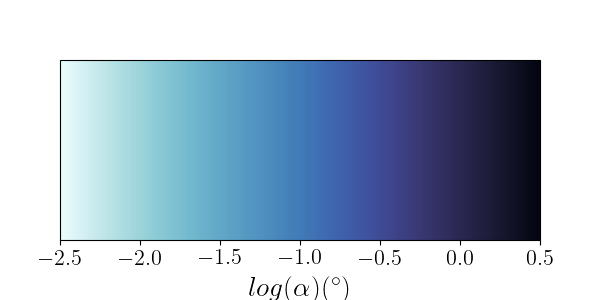
\includegraphics[width=0.7\textwidth,trim={1cm 0cm 1cm 5cm}, clip]{Figures/colorbar_slope.png}
    \end{minipage}
    \caption{Vertical profile of (a,b) heat flux and (c,d) momentum flux averaged over the last inertial period for (a,c) temperature cases and (b,d) slope cases. Momentum flux is expressed in two components:  $\overline{u'w'}$ (dashed) and $\overline{v'w'}$ (solid).} %Change the time interval in (b) back 2h to match (a)
    \label{fig:flux_profiles}
\end{figure}

\begin{figure}
    \centering
    \begin{minipage}{0.5\textwidth}
        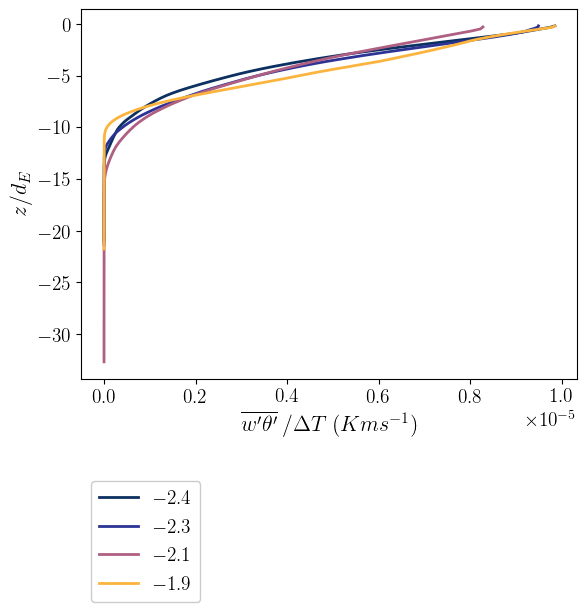
\includegraphics[trim={0 4cm 0 0},clip,width=\textwidth]{Figures/heatflux_cmp_dT_43h_tav13_dTscale_z_profile.png}
    \end{minipage}%
    \begin{minipage}{0.5\textwidth}
        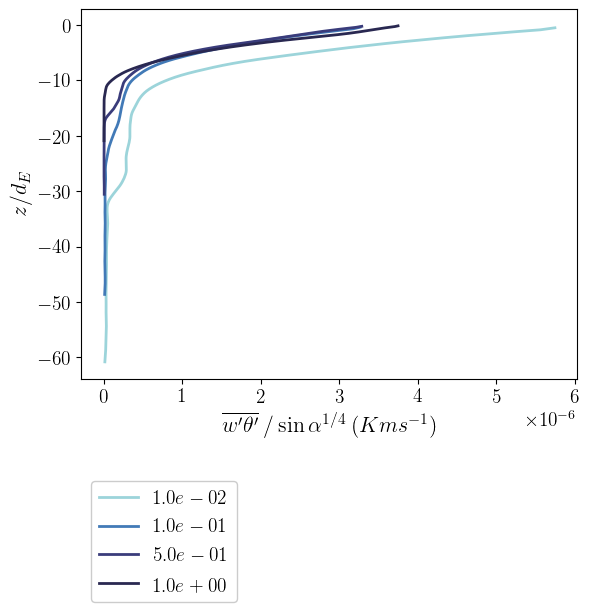
\includegraphics[trim={0 4cm 0 0},clip,width=\textwidth]{Figures/heatflux_cmp_slope_46h_tav13_slopescale_z_profile.png}
    \end{minipage}
    \begin{minipage}{0.5\textwidth}
        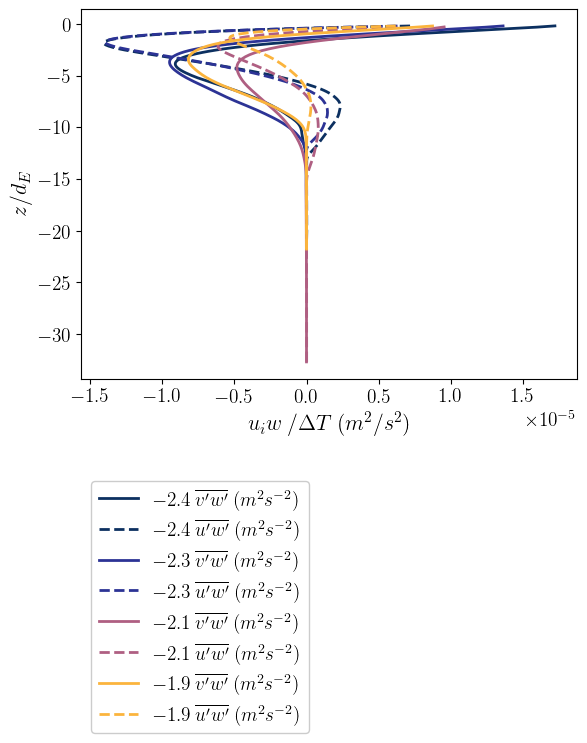
\includegraphics[trim={0 7.5cm 0 0},clip,width=\textwidth]{Figures/momflux_cmp_dT_43h_tav13_dTscale_z_profile.png}
        \centering 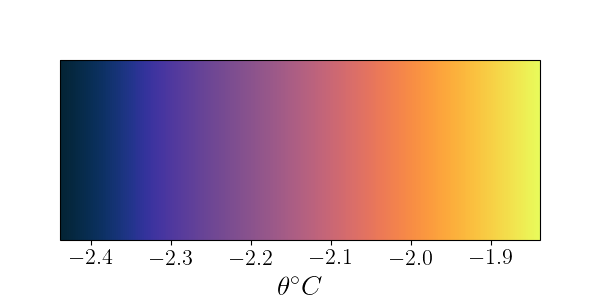
\includegraphics[width=0.7\textwidth,trim={1cm 0cm 1cm 5cm}, clip]{Figures/colorbar_thermal_driving.png}
    \end{minipage}%
    \begin{minipage}{0.5\textwidth}
        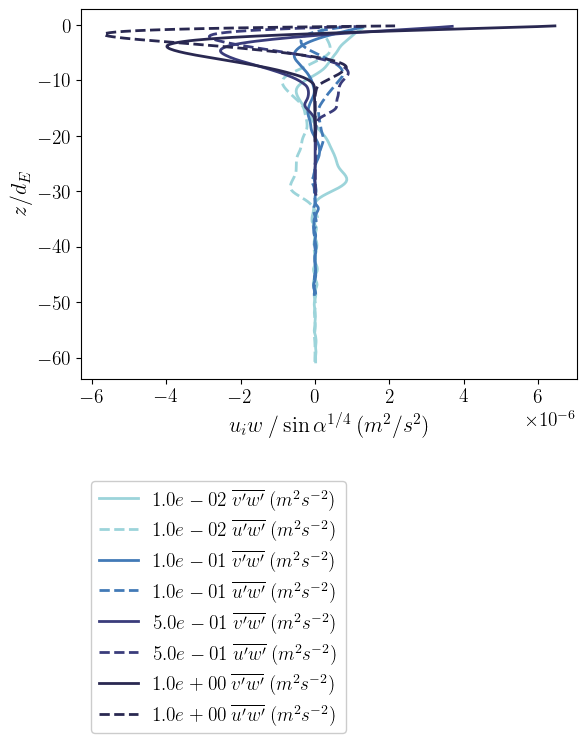
\includegraphics[trim={0 7.5cm 0 0},clip,width=\textwidth]{Figures/momflux_cmp_slope_46h_tav13_slopescale_z_profile.png}
        \centering 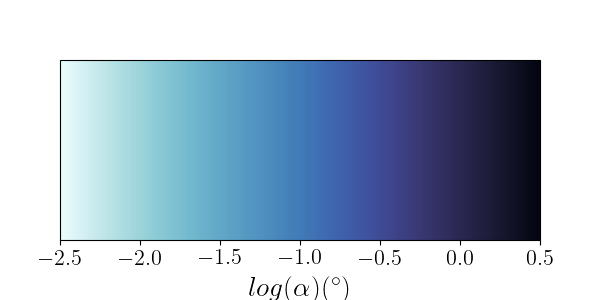
\includegraphics[width=0.7\textwidth,trim={1cm 0cm 1cm 5cm}, clip]{Figures/colorbar_slope.png}
    \end{minipage}
    \caption{Scaled vertical profile of (a,b) heat flux and (c,d) momentum flux averaged over the last inertial period for (a,c) temperature cases and (b,d) slope cases. Momentum flux is expressed in two components:  $\overline{u'w'}$ (dashed) and $\overline{v'w'}$ (solid).} 
    %Change vertical axis limits
    %Change all to centered on 43h and averaged 13h
    \label{fig:Scaled_flux_profiles}
\end{figure}

\begin{figure}[H]
    \centering
    \begin{minipage}{0.5\textwidth}
        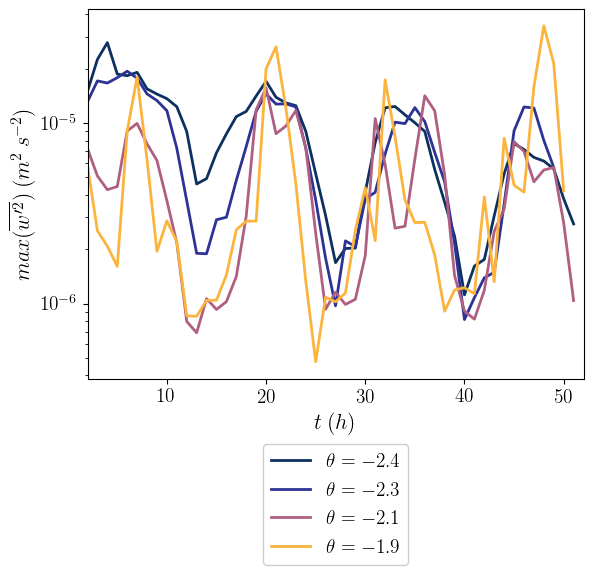
\includegraphics[width=\textwidth]{Figures/w2_max_cmp_dT_t.png}
    \end{minipage}%
    \begin{minipage}{0.5\textwidth}
        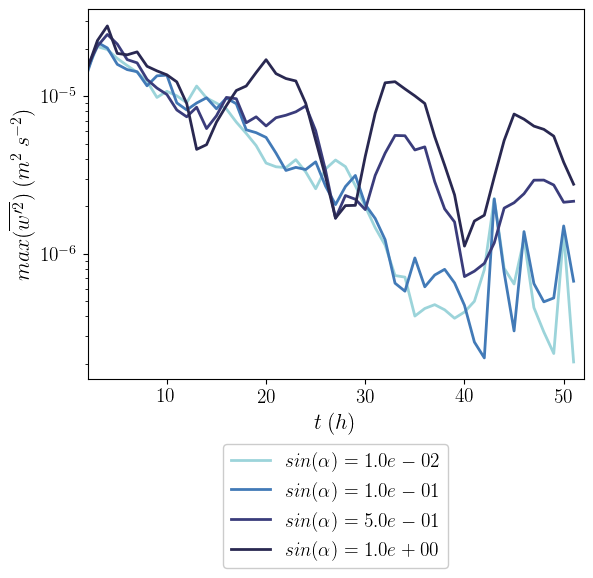
\includegraphics[width=\textwidth]{Figures/w2_max_cmp_dalpha_t.png}
    \end{minipage}
    \caption{Timeseries of maximum vertical velocity fluctuation per hour for (a) thermal driving cases and (b) slope cases.}
    \label{fig:max_w2_timeseries}
\end{figure}

\begin{figure}[H]
    \centering
    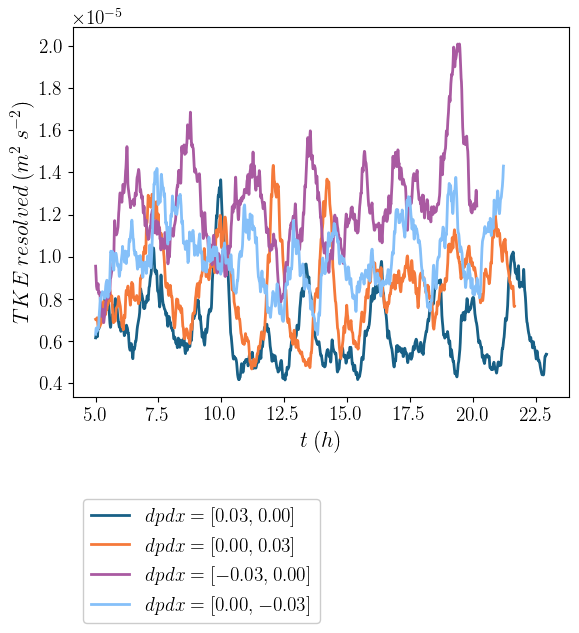
\includegraphics[width=0.5\textwidth]{Figures/e_res_cmp_dpdy_dpdx_t.png}
    \caption{Resolved turbulent kinetic energy as a function of pressure gradient orientation under 0.1$^{\circ}$ slope.}
    \label{fig:e_orientation}
\end{figure}

\begin{figure}[H]
    \centering
    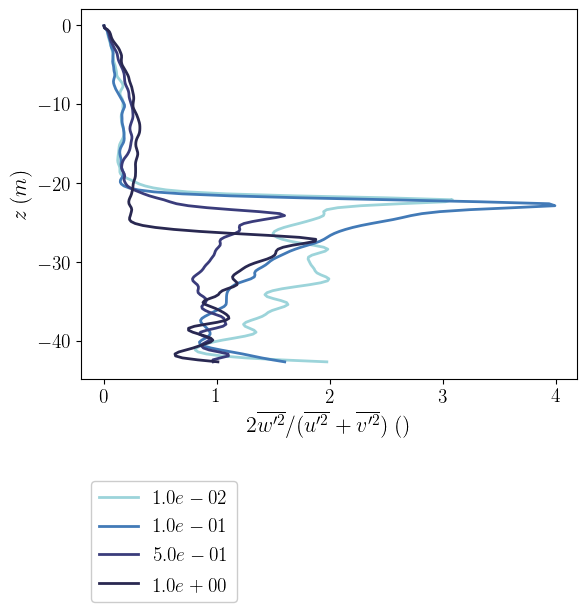
\includegraphics[width=0.5\textwidth]{Figures/vel_var_ratio_cmp_dslope_40hr_tav1_z_profile.png}
    \caption{Ratio of vertical to horizontal velocity variance for slope-varying simulations.}
    \label{fig:vel_var_ratio}
\end{figure}

\begin{figure}[H]
    \centering
    \begin{minipage}{0.5\textwidth}
        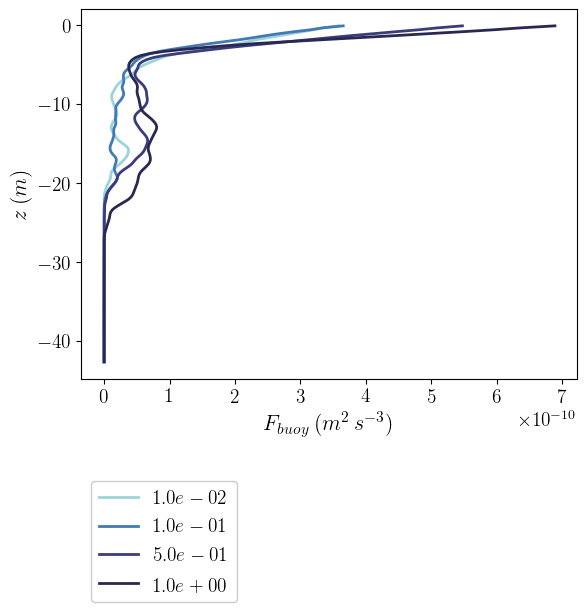
\includegraphics[trim={0 4.5cm 0 0},clip, width=\textwidth]{Figures/Fbuoy_cmp_dslope_40hr_tav1_z_profile.png}
    \end{minipage}%
    \begin{minipage}{0.5\textwidth}
        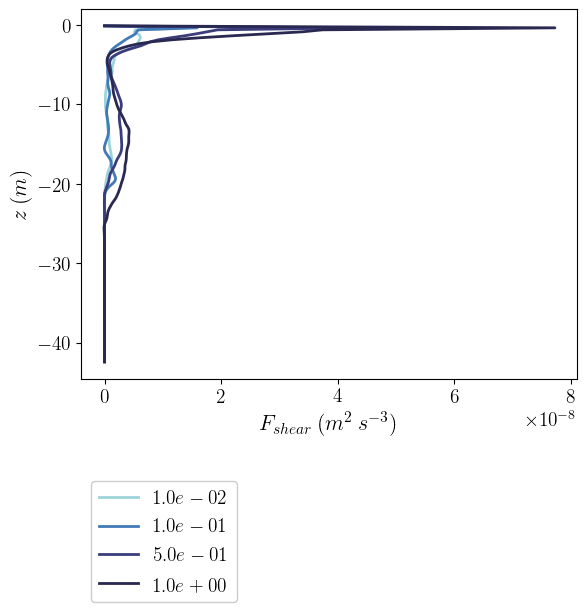
\includegraphics[trim={0 4.5cm 0 0},clip, width=\textwidth]{Figures/Fshear_cmp_dslope_40hr_tav1_z_profile.png}
    \end{minipage}
    \caption{TKE production by (a) buoyancy and (b) shear for slope-varying simulations.}
    \label{fig:tke}
\end{figure}

\begin{figure}[H]
    \centering
    \begin{minipage}{0.5\textwidth}
        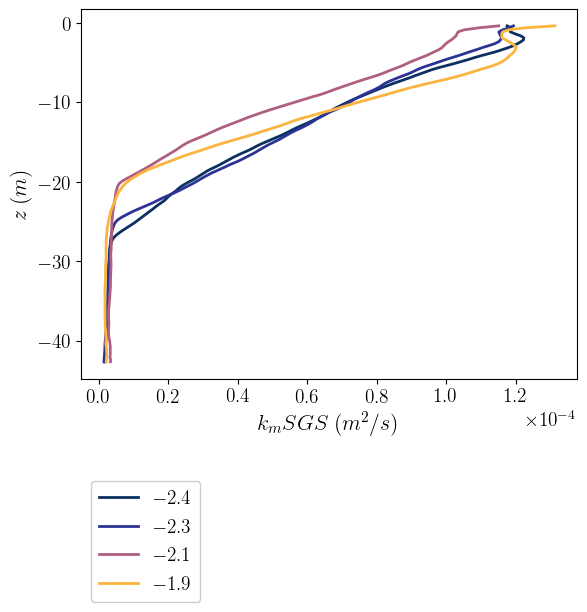
\includegraphics[trim={0 4.5cm 0 0},clip, width=\textwidth]{Figures/km_cmp_dT_44h_tav12_z_profile.png}
    \end{minipage}%
    \begin{minipage}{0.5\textwidth}
        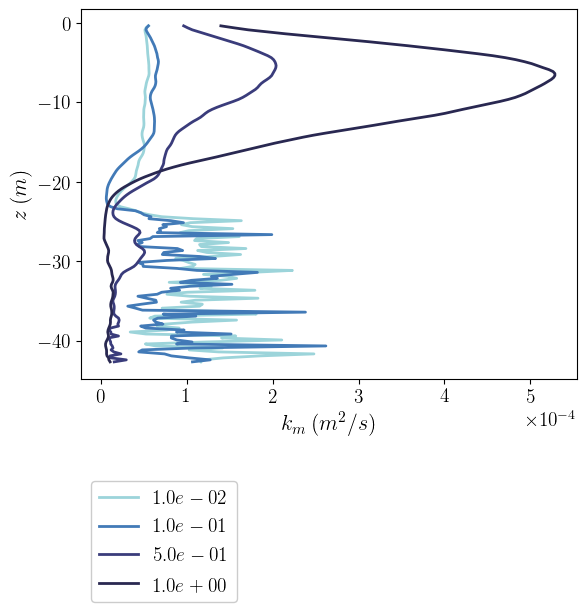
\includegraphics[trim={0 4.5cm 0 0},clip, width=\textwidth]{Figures/km_cmp_slope_46h_tav12_z_profile.png}
    \end{minipage}
    \caption{Effective vertical diffusivity for momentum flux from (a) thermal driving simulations and (b) slope-varying simulations.}
    \label{fig:km}
\end{figure}

\linenumbers
\draftfalse
\journalname{JGR: Oceans}

\begin{document}
%\title{Large-eddy simulations of the ice-shelf oceanic boundary layer}

\correspondingauthor{Carolyn Begeman}{cbegeman@lanl.gov}
\authors{Carolyn Branecky Begeman\affil{1},Xylar Asay-Davis\affil{1}, and Luke Van Roekel\affil{1}}
	
\affiliation{1}{Los Alamos National Laboratory, Los Alamos, New Mexico, USA}

\begin{keypoints}
\item 
\item 
\item 
\end{keypoints}

\begin{abstract}
Xabstract
    
\textbf{Plain language summary}\\
    
\end{abstract}
\newpage

\title{Large-eddy simulations of the ice-shelf oceanic boundary layer}

\correspondingauthor{Carolyn Begeman}{cbegeman@lanl.gov}
\authors{Carolyn Branecky Begeman\affil{1},Xylar Asay-Davis\affil{1}, and Luke Van Roekel\affil{1}}
	
\affiliation{1}{Los Alamos National Laboratory, Los Alamos, New Mexico, USA}

\begin{keypoints}
\item 
\item 
\item 
\end{keypoints}

\begin{abstract}
Small scale, turbulent flow below ice shelves is regionally isolated and difficult to measure and simulate.  Yet these small scale processes, which regulate heat transfer between the ocean and ice shelves, can have global-scale climate impacts; small increases in ice shelf melting decrease the ability of Antarctic ice shelves to “buttress” ice flux to the ocean, potentially allowing for runaway ice loss and sea-level rise. Direct measurements of ocean properties below ice shelves are exceedingly rare, expensive to perform, and difficult to generalize to larger areas. Further, the few available measurements indicate that existing boundary layer theory on sub-ice-shelf turbulence (based largely on observations below sea ice) is incomplete. A fundamental understanding of turbulent flow in this unusual regime is lacking, despite widespread adoption and application of existing parameterizations by the international ocean, ice sheet, and ESM communities.
    
\textbf{Plain language summary}\\
    
\end{abstract}
\newpage
\section{Introduction}

\paragraph{}
The largest source of uncertainty in future sea level rise is the potential loss of ice from the Antarctic Ice Sheet. The rate of grounded ice loss is highly sensitive to the melting of ice shelves, which drain over 80\% of Antarctica’s grounded ice. The Ice-Ocean Boundary Layer (IOBL) controls ice-shelf melting by regulating oceanic heat and salt fluxes to the ice shelf base. Thus, accurate predictions of ice-shelf melting depend on capturing the turbulent dynamics of the IOBL. This representation is also critical for evaluating the sensitivity of the coupled land-ice ocean system. 

\paragraph{}
The sensitivity of ice-shelf melting to increasing seawater temperature, a trend observed along a wide swath of the West Antarctic coastline and a potential trigger for West Antarctic Ice Sheet collapse. 

\paragraph{}
One indication that ocean models do not capture these dynamics is that the modeled thickness of the IOBL differs significantly between ocean models and with model resolution. Furthermore, ocean models predict ice-shelf melting using parameterizations that neglect the buoyancy of the IOBL. This model deficiency likely biases turbulent fluxes through the IOBL and sub-ice-shelf ocean circulation, which is primarily driven by the buoyant flow of water freshened by ice-shelf melting. A new parameterization of ice-shelf melting that accounts for boundary layer dynamics is needed to achieve a more physically-based, accurate coupling of ice sheets and oceans in climate models.

\paragraph{}
In this study, we model turbulent heat, salt, and momentum fluxes through the IOBL using Large-Eddy Simulation (LES). Whereas ocean models typically used to model sub-ice-shelf ocean cavities cannot capture the relevant turbulent scales for boundary layer dynamics, LES captures the dominant energy-containing scales of turbulence and represents smaller, unresolved scales with varying degrees of complexity. An effective parameterization of ice-shelf melting is likely to depend on ice-shelf slope, the temperature, salinity, and velocity outside the IOBL, and the depth of the ice-ocean interface. We vary these parameters between model runs and characterize turbulent fluxes, IOBL thickness, and ice-shelf melt rates.  

\paragraph{}
Characterizing turbulence in the presence of a buoyancy flux and sloping boundary is a fundamental problem in fluid dynamics. 

\section{Methods}

\paragraph{The PALM model}
The PArallelized Large eddy simulation Model (PALM) was developed at the Institute of Meteorology and Climatology at Leibniz Universitat Hannover (Germany). It has been applied to the simulation of atmospheric and ocean boundary layers. However, it has never been used specifically to treat a sub-ice-shelf ocean boundary layer. For this application, the key model development was the implementation of dynamic melting fluxes. 

\subsection{Governing equations}

%Mass conservation for incompressible flows
%\begin{equation} \label{eq:volconserv}
%\frac{\partial u_j}{\partial x_j} = 0
%\end{equation}
%The model enforces incompressibility with 
%\begin{equation} \label{eq:pdiv}
%\frac{\partial^2 \pi^{*t}}{\partial x_i^2} = \frac{\rho_0}{\Delta t} \frac{\partial u_{i,pre}^{t + \Delta t}}{\partial x_i}
%\end{equation}

Prognostic equations:
Momentum conservation
\begin{equation} \label{eq:uprog}
	\frac{\partial u_i}{\partial t} = 
	-\frac{\partial u_i u_j}{\partial x_i}
	-\varepsilon_{ijk} f_j u_k 
	+ \varepsilon_{i3j} f_3 u_{g,j} 
    + g_i \frac{\rho - \rho_a}{\rho_0}
	- \frac{1}{\rho_0}\frac{\partial \pi^*}{\partial x_i}
	- \frac{\partial}{\partial x_j}(\overline{u''_i u''_j} - \frac{2}{3}e\delta_{ij})
	- \frac{\tau_i}{\rho}
\end{equation}
	
The terms on the right hand side of Equation \ref{eq:uprog} are, in order: advection, Coriolis forcing, imposed geostrophic flow, buoyancy forcing, a correction for divergence in the flow (imposing incompressibility), and sub-grid scale momentum fluxes. 
% Prognostic equation for Resolved TKE
% \begin{equation} \label{eq:eprog}
% \frac{\partial e^*}{\partial t} = 
% -u_j \frac{\partial e^*}{\partial x_j} 
% - (\overline{u^*_i u^*_j})\frac{\partial u_i}{\partial x_j} + \frac{g_i}{\rho_0}\overline{u^*_i \rho^*}
% \end{equation}

%\paragraph{}% Sloping surface
We represent a sloping ice base by rotating the gravity and Coriolis vectors while keeping the domain a rectangular prism. 
%In PALM v0 the buoyancy terms were based only on temperature rather than density. 
Thus, 
\begin{equation} \label{eq:g}
	%\textbf{g} = g [sin \alpha,0,cos \alpha]
	\textbf{g} = g [sin \alpha sin \beta,cos \beta,cos \alpha]
\end{equation}
\begin{equation} \label{eq:f}
    \textbf{f} = 2 \Omega [sin \phi sin \alpha,cos \phi,sin \phi cos \alpha]
\end{equation}
$\beta$ is the angle the slope direction makes with north.
$\alpha$ is the slope angle from horizontal
$\phi$ is the latitude.
The ice base always slopes in the positive x-dimension of our domain or east, thus $\beta = 0$. 

The buoyancy term in Equation \ref{eq:uprog} combines the contributions of along-slope pressure gradient due to the slope of the ice shelf in hydrostatic equilibrium and buoyancy due to changes in density. The along-slope pressure gradient is set by the ambient density of the water column $\rho_a$. This ambient density is determined using the initial far-field ocean density. For a non-sloping domain, $\rho_a$ = $\rho_i$
% the far-field density remains constant during the simulation due to relaxation boundary conditions
% temperature and salinity values and the initial vertical hydrostatic pressure profile in the middle of the domain. 
%Thus, we assume that the evolution of density in the boundary layer does not significantly affect buoyancy/ice-shelf slope. 
We neglect hydrostatic pressure gradients along slope. For the maximum slope simulated in this study, the maximum hydrostatic pressure gradient is on the order of 1 bar m\textsuperscript{-1}. % or 10 pa/m
This simplification has the advantage of avoiding pressure discontinuities across periodic boundary conditions. 
%We assume that density differences between ambient and simulated conditions does not significantly change as a function of along-slope pressure changes. 
% \begin{equation}
%     \rho(T(x,z),S(x,z),p(x,z)) - \rho_a(T_a,S_a,p(x,z)) \approx 
%     \rho(T(x,z),S(x,z),p(x_{mid},z) - \rho_a(T_a,S_a,p(x_{mid},z))
% \end{equation}
%These density differences are verified to be within XX $kg/m^3$ for these simulations. 

%\paragraph{}%Surface drag
The last term in Equation \ref{eq:uprog} represents the loss of momentum due to drag between the ice surface and the flow, where $\tau$ is the shear stress. This term is parameterized by the sub-grid scheme.

Heat and salt conservation
\begin{equation} \label{eq:ptprog}
\frac{\partial \theta}{\partial t} = -\frac{\partial u_j \theta}{\partial x_j} - \frac{\partial}{\partial x_j}(\overline{u'_i \theta'}) % - F_T
\end{equation}

\begin{equation} \label{eq:saprog}
\frac{\partial S}{\partial t} = -\frac{\partial u_j S}{\partial x_j} - \frac{\partial}{\partial x_j}(\overline{u'_i S'})
\end{equation}

Dynamic ice melting influences these equations through a modification to the SGS vertical fluxes of heat and salt at the top of the model domain, discussed XX.

\subsection{Turbulence closure}\label{meth:tcm}

The turbulence closure scheme is Anisotropic Minimum Dissipation (Rozema) employing the extension to scalars introduced by Abkar and Moin. Our implementation shows similar qualitative behavior to the stable atmospheric boundary layer published in XX; some inter-model variability is expected due to different numerics.

Momentum fluxes are parameterized according to law of the wall following a linear stability function as in Vreugdenhil and Taylor (2019):

\begin{equation}
    \vec{\tau} = \rho \overline{\vec{u}'w'} = \rho u_* \frac{ \kappa (u(z_1) - u_b}{\textrm{ln}(z_1/z_0)-\Psi_m(\zeta_1)}
\end{equation}

where $\zeta_k = z_k/L_O$, friction velocity $u_*$, $z_0$ is the roughness length, and $z_1$ is the evaluation depth at the uppermost grid cell.
\begin{equation}
    \Psi_m(\zeta) = 1 + \beta_m \zeta
\end{equation}

Similarly the sub-grid fluxes of scalars are parameterized
\begin{equation}
    \overline{w'\theta'} = \Gamma_{\theta} u_* (\theta(z_1) - \theta_b),\: 
    \overline{w'S'} = \Gamma_S u_* (S(z_1) - S_b)
\end{equation}

\begin{equation}
    \Gamma_{\theta}^{-1} = (\Gamma_{\theta,turb} + \Gamma_{\theta,mol})^{-1},\:
    \Gamma_S^{-1} = (\Gamma_{S,turb} + \Gamma_{S,mol})^{-1}
\end{equation}

\begin{equation}
    \Gamma_{\theta,turb} = \kappa^{-1} (\textrm{ln}(z_1/z_0) - \Psi_{\theta}(\zeta_1))
    % + \Psi(z_0/L_O)) % correction for roughness length
\end{equation}
\begin{equation}
    \Gamma_{S,turb} = \kappa^{-1} (\textrm{ln}(z_1/z_0) - \Psi_S(\zeta_1))
    % + \Psi(z_0/L_O)) % correction for roughness length
\end{equation}
If a portion of the ice face experiences freezing, $\Gamma_\theta$ and $\Gamma_S$ are set to a higher value indicating destabilizing fluxes ($Gamma_{f}$, Table \ref{table:var}).

\begin{equation}
    \Psi_{\theta,S}(\zeta) = 1 + \beta_{\theta,S} \zeta
\end{equation}
The coefficients of these stability functions are chosen as in Wyngaard 2010; Zhou et al. 2017 (Table \ref{table:var}.


\begin{equation}
    \Gamma_{\theta,mol} = 12.5 \textrm{Pr}^{2/3} - 6
\end{equation}
\begin{equation}
    \Gamma_{S,mol} = 12.5 \textrm{Sc}^{2/3} - 6
\end{equation}
where Pr is the Prandtl number and Sc is the Schmidt number. %similarly for $\Gamma_{S,mol}$ but with Schmidt number.

We use ``virtual" freshwater fluxes as opposed to freshwater fluxes with mass or volume; thus, the scalar fluxes take the form \cite{XX}
\begin{equation}
    \overline{w'\theta'} = -c_p u_*
    (\Gamma_{\theta} - \Gamma_S \frac{S_b - S_1}{S_b})(\theta_b-\theta)
    %\rho_{sw}\overline{w'\theta'} = c_p(\rho_{sw} \Gamma_T u_* + \rho_{fw} m)(T(z_1) - T_b)
\end{equation}

\begin{equation}
    \overline{w'S'} = -u_*
    (\Gamma_S - \Gamma_S \frac{S_b - S_1}{S_b})(S_b-S)
    %\rho_{sw}\overline{w'S'} = (\rho_{sw} \Gamma_S u_* + \rho_{fw} m)(S(z_1) - S_b)
\end{equation}

%\subsection{Prognostic melt calculation}
The temperature and salinity at the ice-ocean interface, $\theta_b$ and $S_b$, are unknown. Three equations are used to solve for these quantities and the melt rate, the so-called three-equation parameterization:

\begin{equation}\label{eq:melt_1}
    \rho c_p \overline{w'\theta'}_b = -\rho_f m L_i
    %\rho c_p \overline{w'\theta'}_b - F_{T,cond} = -\rho_{fw} m L_i
\end{equation}

\begin{equation}\label{eq:melt_2}
    \rho \overline{w'S'}_b = −\rho_f m S_b
\end{equation}

\begin{equation}\label{eq:melt_3}
    \theta_b = \theta_f(p,S_b)
\end{equation}

These equations specify that heat and salt are conserved at the ice-ocean interface (Equations \ref{eq:melt_1} and \ref{eq:melt_2})and the interface temperature is fixed at the local freezing temperature using the polynomial function from \cite{jackett_2006} (Equation \ref{eq:melt_3}). Equation \ref{eq:melt_1} assumes that the conductive heat flux into ice is 0.
% short version in A01

\subsection{Simulation set-up}

The domain is a 64 m$^3$ cube with horizontal resolution of 0.5 m and vertical resolution of 0.25 m. The ice-ocean interface is located on the top boundary of the domain. Large-scale horizontal pressure gradients drive the mean flow, which is geostrophic in the far-field where buoyancy does not modify the flow. We choose a pressure of 800 dbar at the top of the domain, a rather arbitrary choice given that the depth of ice shelf bottoms ranges an order of magnitude (roughly -2000 m to -200 m). The potentially dynamically relevant differences between conducting these simulations at surface pressure and 800 dbar is that the first derivative of the freezing temperature with respect to salinity is 20\% smaller and the first derivative of density with respect to salinity is about 100\% larger.

%\paragraph{Initial and boundary conditions}
Boundary conditions for velocity, temperature and salinity are cyclic at the side boundaries, Dirichlet at the bottom boundary, and von Neumann at the top boundary. The bottom third of the domain is a sponge layer within which velocity, temperature, and salinity are relaxed toward their assigned values at the bottom of the domain. The sponge layer results in no vertical fluxes of heat, salt, or momentum across the bottom boundary. The von Neumann boundary conditions at the top of the domain correspond to the sub-grid fluxes of heat, salt and momentum (Equations XX), as resolved fluxes go to zero at a no-penetration boundary. The drag coefficient for all simulations is 0.003, a canonical value below sea ice and ice shelves though poorly constrained \cite{XX}. The drag coefficient sets the roughness length $z_0$ in the boundary flux equations of Section \ref{sec:meth_sgs} through the quadratic drag ``law of the wall." A complete list of parameter choices can be found in Table \ref{table:var}.

There are two sets of simulations which have a base case in common. The base case has low far-field thermal driving of 0.1 $^{\circ}$C and a relatively high slope for Antarctic ice shelves of 1$^{\circ}$ and vigorous far-field geostrophic flow of 20 cm s$^{-1}$ generated by a 0.03 pressure gradient. These conditions were chosen to favor a high TKE regime, for reasons discussed in Section \ref{sec:disc}. To examine the relationship between thermal driving and melt rate, as well as turbulent flow characteristics, we vary the far-field thermal driving from 0.1 $^{\circ}$C to 0.5 $^{\circ}$C in the first set of simulations. In the second set of simulations we reduce the slope from 1$^{\circ}$ to 0.01$^{\circ}$. 

The far-field salinity for all runs is 35 g kg\textsuperscript{-1}. Initially, both temperature and salinity increase with depth over the upper two-thirds of the domain. The background salinity stratification dominates the density stratification, with an inverse stability ratio $R_\rho^*$ of 20. 

The simulation duration is 50 h, corresponding to a little over 4 inertial periods. By this point, the turbulent intensity as measured by the maximum vertical velocity fluctuation, is reasonably steady-state over one inertial period for the 1$^{\circ}$-slope simulations (Figure S\ref{fig:max_w2_timeseries}). The turbulent intensity for cases with slopes less than 1$^{\circ}$ continues to decline, as we discuss later.

\section{Results}

% Melt sensitivity to thermal driving
Melt rates decline over the course of the simulations (Figure \ref{fig:melt_timeseries}), preventing the identification of steady-state melt rates. 
This decline is in response to a co-committent increase in stratification during the course of the simulation, which decreases vertical heat fluxes by reducing vertical turbulent fluctuations (Fig. S\ref{fig:max_w2_timeseries}). We do not continue our simulations in the hope of reaching steady-state conditions because the increase in stratification reduces the turbulent length scales and necessitates higher model resolution than we have used here. The high thermal driving case approaches steady-state more rapidly than low thermal driving cases due to increased shear production of TKE from the buoyant acceleration of the IOBL.

% Melt rate relationship with inertial period
The dominant temporal frequency in melt rate is the inertial frequency; however, the melt response to those oscillations is highly nonlinear. Maximum melt rates occur when the mean flow is oriented between the up-slope direction and the Coriolis-favored direction, and minimum melt rates roughly 180$^{\circ}$ opposed to that. Melt rate fluctuations increase as thermal driving increases, which we attribute to the increasing importance of buoyancy forcing in driving a near-boundary plume and thus determining the depth-distribution of shear. During high-melt periods, the far-field flow is oriented up-slope and shear production of TKE is concentrated near the boundary. During low-melt periods, the far-field flow is oriented down-slope and shear production of TKE is concentrated a few meters away from the boundary. The vertical heat flux profile through the water column follows the profile of shear production of TKE (Fig. \ref{fig:dT_profiles}, Fig. S\ref{fig:TKE_balance}). The low-melt period is somewhat brief, roughly 1/4 of the inertial period, as the onset is delayed by the time it takes to increase near-boundary stratification. In simulations where the background pressure gradient orientation was varied, we also observe reduced TKE when the mean flow is down-slope, suggesting this relationship is not unique to inertial oscillations but is more closely related to the vertical velocity structure and the depth of maximum shear. (Fig. S\ref{fig:e_orientation}).

The time-averaged melt rates are roughly linear with thermal driving (Figure \ref{fig:melt_sensitivity}a). The thermal exchange coefficient as computed using Equation \ref{eq:gamma} during the last 12 hours of the simulations is between 0.005 and 0.006 for the simulated range of thermal driving values. The time-averaged value decreases somewhat in the high thermal driving cases due to pronounced periods of low melt as TKE declines with increasing stratification. 

These values are less than the thermal exchange coefficient of 0.011 derived from observations in Jenkins et al. (2010). During the first 12 hours of the simulation, simulated thermal exchange coefficients are 0.008 due to weaker stratification near the interface and higher friction velocities due to greater TKE. 

Boundary layer depths as characterized by a peak in the ratio of vertical to horizontal velocity variance range from 15 m to 25 m for the moderate to low thermal driving cases.

In these simulations we find that the destruction of TKE by the stabilizing buoyancy flux is two orders of magnitude smaller than shear production of TKE. Given that the background flow is relatively strong for ice shelf settings, this result may be only narrowly applicable. However, it is consistent with \citep{davis_nicholls} who found that shear production was an order of magnitude greater than buoyancy destruction of TKE in the IOBL below Larsen C Ice Shelf. 



% Description of simulation features

\begin{figure}
    \centering
    \begin{minipage}{0.5\textwidth}
        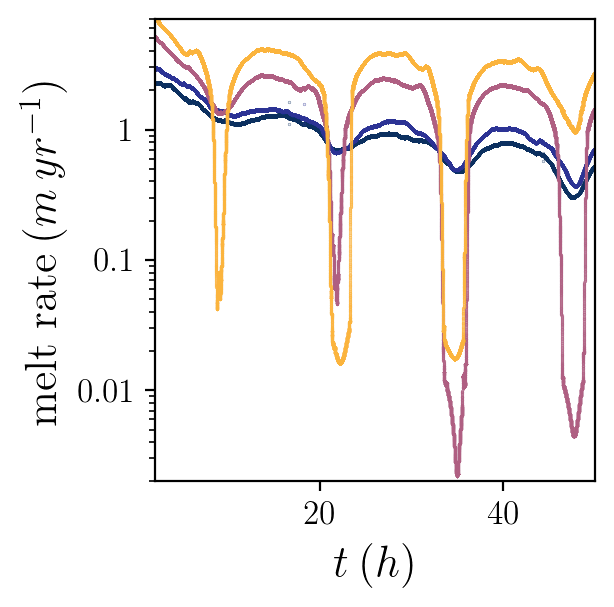
\includegraphics[width=\textwidth]{Figures/melt_cmp_dT_t.png}
    \end{minipage}%
    \begin{minipage}{0.5\textwidth}
        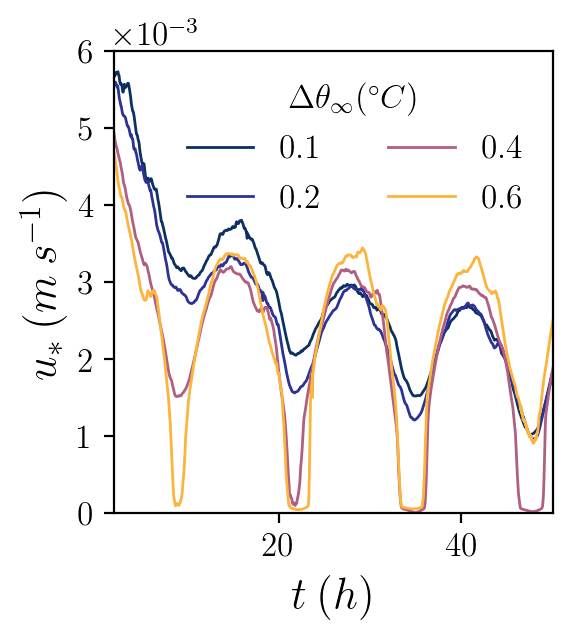
\includegraphics[width=\textwidth]{Figures/us_cmp_dT_t.png}
    \end{minipage}%
    \caption{Thermal driving simulations. (a) evolution of melt rate (b) evolution of friction velocity}
    \label{fig:dT_timeseries}
\end{figure}

\begin{figure}
    \centering
    \begin{minipage}{0.5\textwidth}
        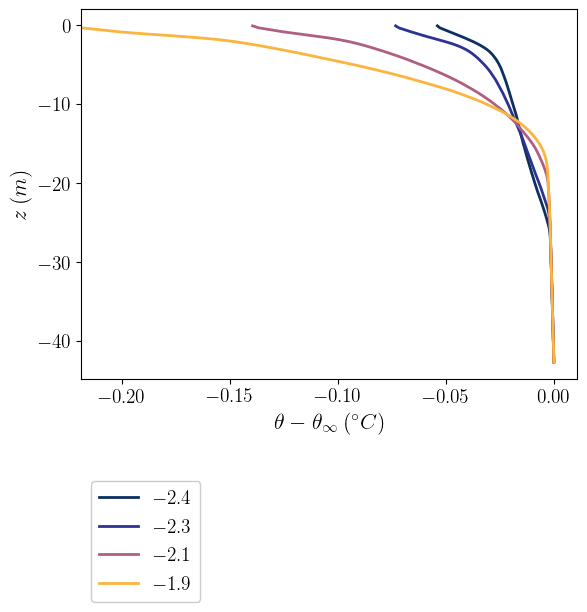
\includegraphics[trim={0 4cm 0 0},clip, width=\textwidth]{Figures/ptfar_cmp_dT_40hr_tav1_z_profile.png}
    \end{minipage}%
    \begin{minipage}{0.5\textwidth}
        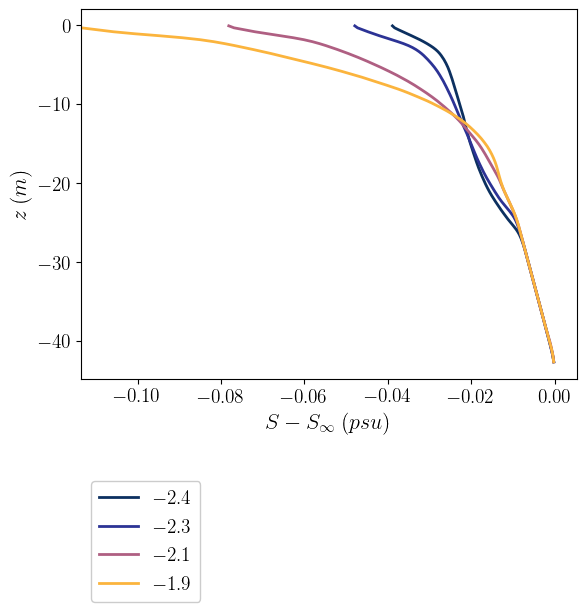
\includegraphics[trim={0 4cm 0 0},clip, width=\textwidth]{Figures/safar_cmp_dT_40hr_tav1_z_profile.png}
    \end{minipage}
    \newline
    \begin{minipage}{0.5\textwidth}
        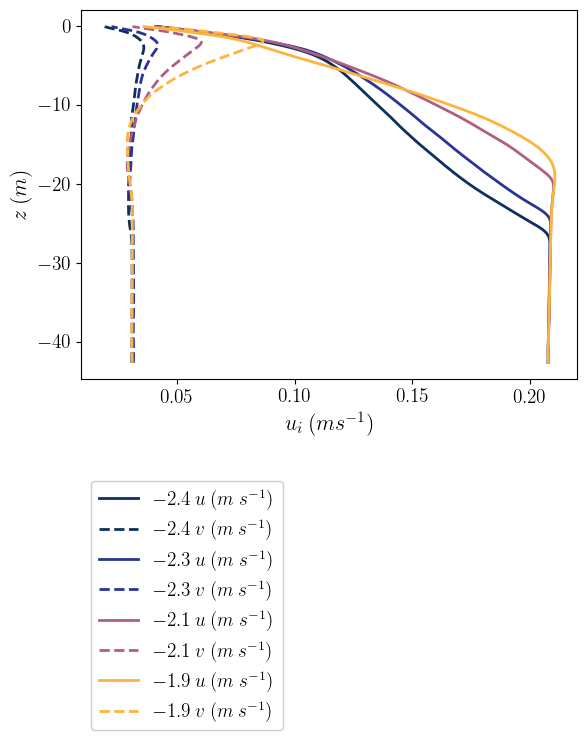
\includegraphics[trim={0 7.5cm 0 0},clip, width=\textwidth]{Figures/velocity_cmp_dT_40hr_tav1_z_profile.png}
    \end{minipage}%
    \begin{minipage}{0.5\textwidth}
        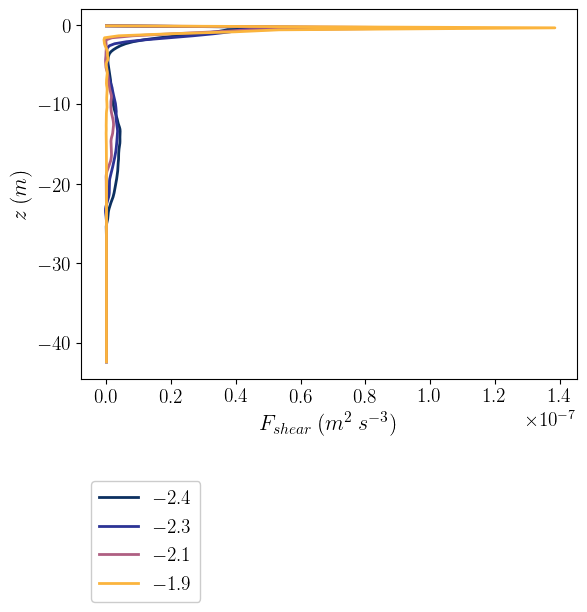
\includegraphics[trim={0 7.5cm 0 0},clip, width=\textwidth]{Figures/Fshear_cmp_dT_40hr_tav1_z_profile.png}
    \end{minipage}
    \newline
    \begin{minipage}{0.5\textwidth}
        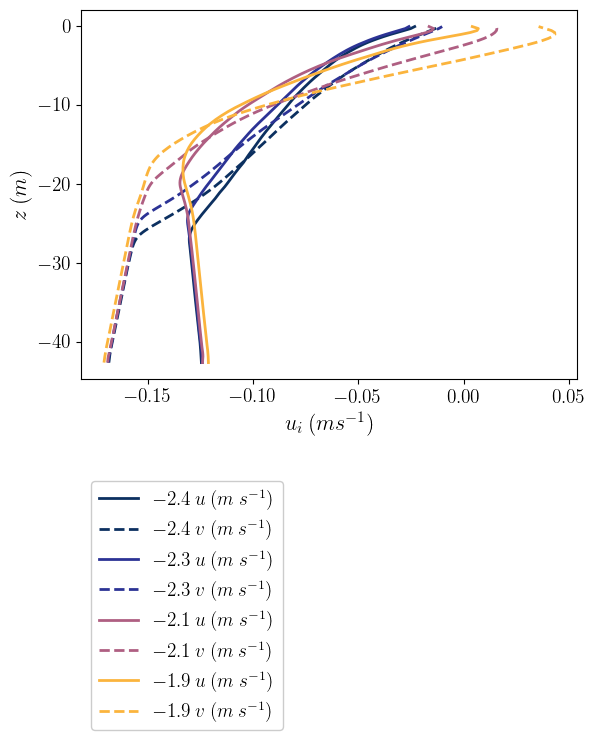
\includegraphics[trim={0 7.5cm 0 0},clip, width=\textwidth]{Figures/velocity_cmp_dT_48hr_tav1_z_profile.png}
    \end{minipage}%
    \begin{minipage}{0.5\textwidth}
        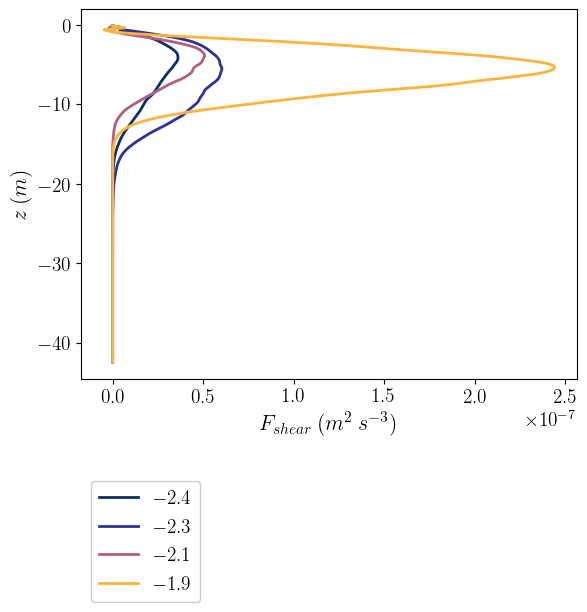
\includegraphics[trim={0 7.5cm 0 0},clip, width=\textwidth]{Figures/Fshear_cmp_dT_48hr_tav1_z_profile.png}
    \end{minipage}
    \caption{Thermal driving simulations. (a) temperature relative to far-field temperature (b) salinity relative to far-field salinity (c) velocity (d) heat flux}
    \label{fig:dT_profiles}
\end{figure}

\begin{figure}
    \centering
    \begin{minipage}{0.5\textwidth}
        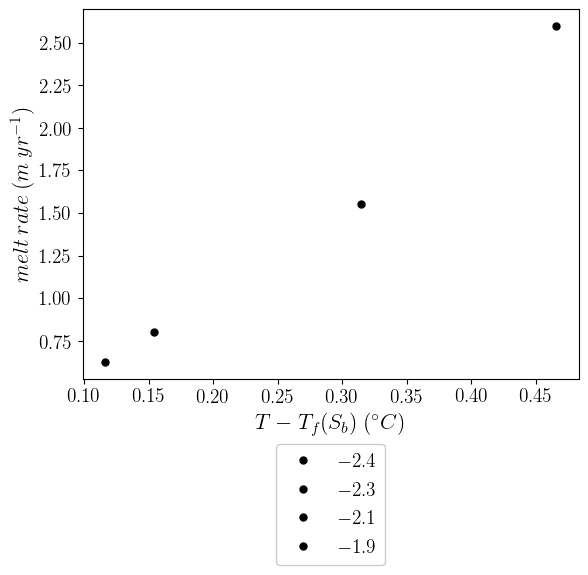
\includegraphics[trim={0 3.5cm 0 0},clip,width=\textwidth]{Figures/melt_dT_tav12.png}
    \end{minipage}%
    \begin{minipage}{0.5\textwidth}
        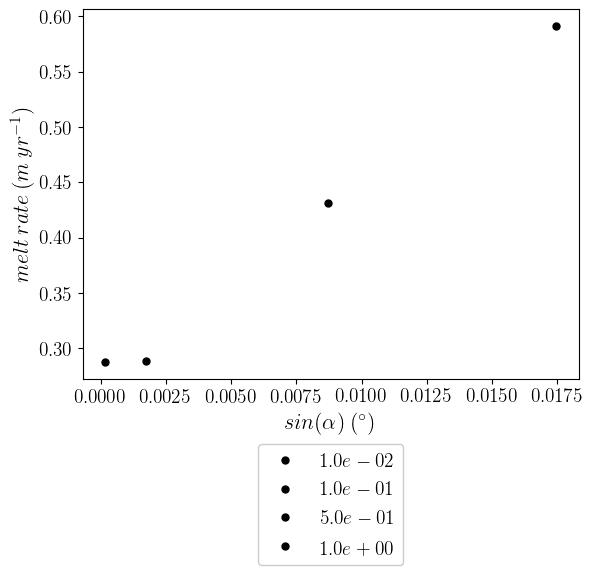
\includegraphics[trim={0 3.5cm 0 0},clip,width=\textwidth]{Figures/melt_dslope_tav12.png}
    \end{minipage}
    \begin{minipage}{0.5\textwidth}
        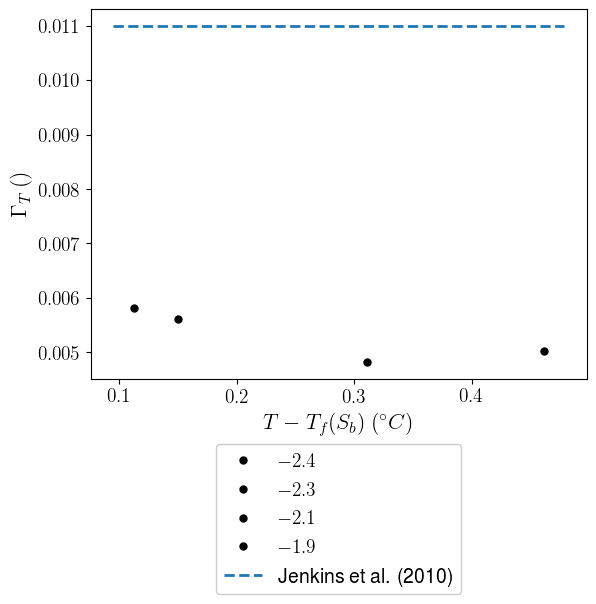
\includegraphics[trim={0 4.1cm 0 0},clip,width=\textwidth]{Figures/gammaT_dT_tav12_zlim2.png}
    \end{minipage}%
    \begin{minipage}{0.5\textwidth}
        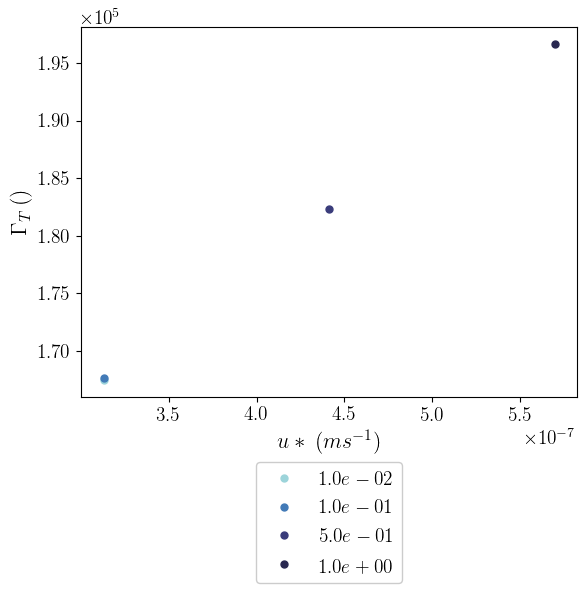
\includegraphics[trim={0 0cm 0 0},clip,width=\textwidth]{Figures/gamma_T__us__dslope_tav12_tlim52.png}
    \end{minipage}
    \caption{(a) Melt rate vs. thermal driving. (b) Melt rate vs. slope. (c) Thermal exchange coefficient vs. far-field thermal driving for thermal driving simulations. (d) Thermal exchange coefficient vs. friction velocity for sloped simulations.}
    \label{fig:melt_sensitivity}
\end{figure}


\section{Discussion}

This is the second LES study of the ice-shelf ocean boundary layer in which the boundary layer turbulence declines throughout the coarse of the simulation \cite{XX}. This results in declining melt rates as well, making it difficult to evaluate the relationship between melting and far-field conditions at steady state -- which has been central to the goal of improving ice-shelf basal melt parameterizations with the results of high-resolution simulations.
There are a few possible explanations for this phenomenon. Perhaps the best candidate is that either the sub-grid scheme or the model numerics are too dissipative, such that the TKE generated by the resolved dynamics is lost too quickly. Another possibility is that we are missing or underestimating a source of TKE in the model. Tides were not in

Furthermore, the simulations shown here have a sufficiently strong salinity gradient that the potential energy stored in the temperature gradient is not converted to TKE. Simulations now shown here suggest that simulated TKE can be maintained when stability ratios are as low as 4, but a detailed exploration of this phenomenon is not within the scope of the current work as LES cannot allow for the development of double-diffusive convection, which may occur when the stability ratio is lower than \~ 10.  
%It appears that well-mixed boundary layers are produced for a narrower range of conditions in simulations than in observations. 

\section{Figures and Tables}

\subsection{Figures}

\subsection{Tables}
    \begin{table}[h]
    \caption{    }
    \label{table:var}
    \begin{center}
    \begin{tabular}{lll}
    \multicolumn{3}{c}{}\\
	% XX consider including:	% businger coefficients
	
	$c_d$           & drag coefficient & 0.003 \\
    $c_p$       & heat capacity of water    & 4218\\   
	$dP/dx,dP/dy$   & horizontal pressure gradients & $0.0,0.03$ Pa m$^{-1}$\\
	$dS/dz$   & far-field vertical salinity gradient & 0.5 PSU km$^{-1}$\\
	$d\theta/dz$   & far-field vertical temperature gradient & 0.1 $^{\circ}$C km$^{-1}$\\
    %$e$         & SGS TKE & \\
    %$e*$        & resolved TKE & \\
	$h_x,h_y$       & domain width              & 64 m\\
	$h_z$           & domain height             & 64 m\\ 
	%$L_O$ & Monin-Obukhov length & \\
    $L_f$           & latent heat of fusion     & $3.3 x 10^5$ XXunits\\
	$P_0$           & domain top pressure          & 800 dbar\\
	$Pr$           & Prandtl number      & 13.8\\
	$rdf$           & rayleigh damping coefficient & 0.001\\
	$S_{\infty}$      & far-field salinity     & $34 - 35$ PSU \\
	$Sc$           & Schmidt number      & 2432\\
	%$z_0$ & roughness length & \\
	%$z_1$ & evaluation depth for melt parameterization & 0.25 m\\
	%Greek letters
	$\alpha$        & *ice shelf slope           & 0.01 -- 1$^{\circ}$ \\
	$\beta$         & angle between vector oriented up-slope and North & 90$^{\circ}$\\% -- 2$\pi$\\
	$\beta_m$         & businger coefficient for momentum & -4.8 \\
	$\beta_{\theta}$         & businger coefficient for temperature & -5.6 \\
	$\beta_S$         & businger coefficient for salinity & -5.6\\
	$\Delta_x,\Delta_y$& horizontal resolution  & 0.5 m\\
	$\Delta_z$      & vertical resolution       & 0.25 m\\
    $\Gamma_f$   & Destabilizing transfer coefficient & $5.7 \times 10^{-3}$\\% \pm 10\%& \makecell[l]{X\% of the domain is freezing \\ for X temperature case}\\ 
	$\phi$ & latitude & -70 S \\
	$\theta_{\infty}$      & *far-field temperature     & $-2.4 - -1.9 ^\circ C$ \\
    \hline
    %\botline % ametsoc
    \end{tabular}
    \end{center}
    \end{table}
    %$L_{O,min}$ & $\Delta z/20$ & \makecell[l]{X\% of the domain reaches $L_O$ minimum \\ for X temperature case} \\
    %$L_{O,max}$ & $20\Delta z$ & \makecell[l]{X\% of the domain reaches $L_O$ maximum \\ for X temperature case}\\ 
    %$z_m$       & max(z(min $d\theta/dz$),z(min $dS/dz$)) & not tested\\ %up to 2 x boundary layer depth

\section{Acknowledgements}

This research used resources provided by the Los Alamos National Laboratory Institutional Computing Program, which is supported by the U.S. Department of Energy National Nuclear Security Administration under Contract No. 89233218CNA000001.

\end{document}